\chapter{Modelling a Database for Dynamic Multimedia Data}
\label{chapter:system_model}

\section{Adaptive Index Management}

\begin{figure}[h!]
    \centering
    \begin{subfigure}[b]{0.40\textwidth}
        \centering
        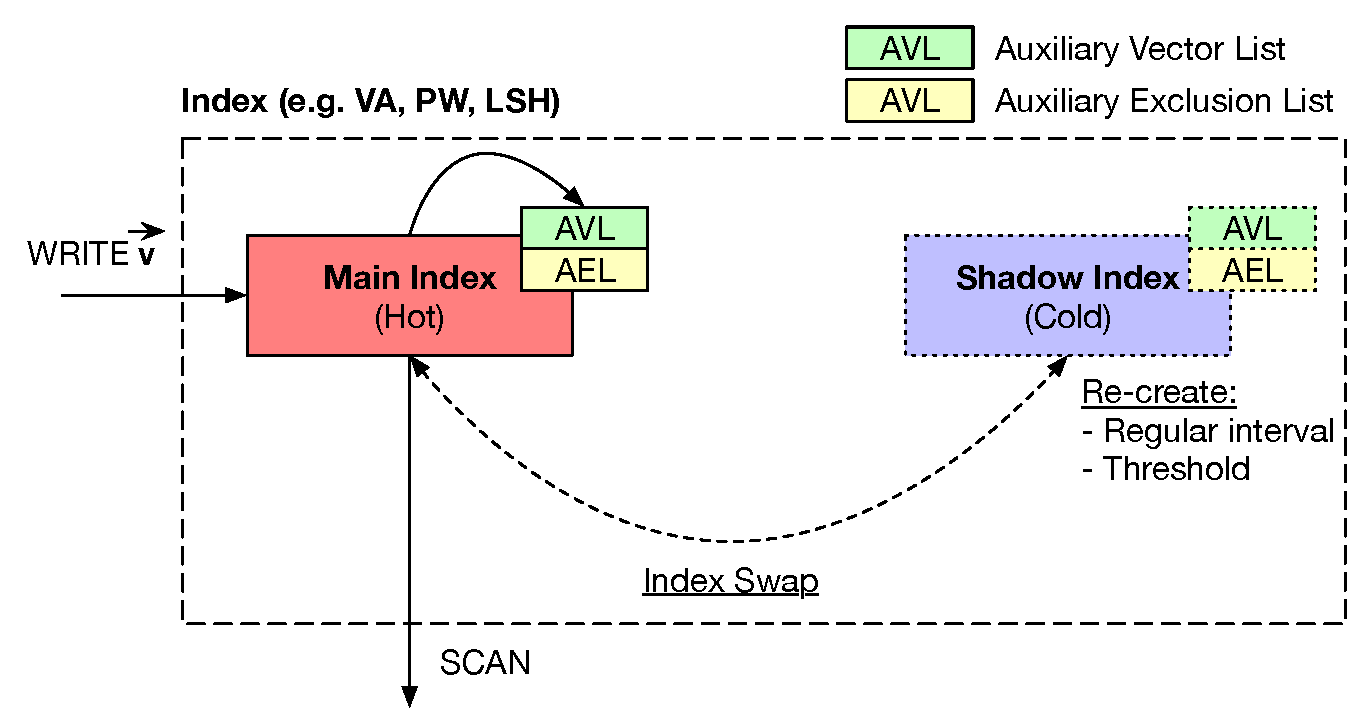
\includegraphics[width=\textwidth]{figures/adaptive_index.eps}
        \label{fig:adaptive_index:architecture}
    \end{subfigure}
    \hfill
    \begin{subfigure}[b]{0.40\textwidth}
        \centering
        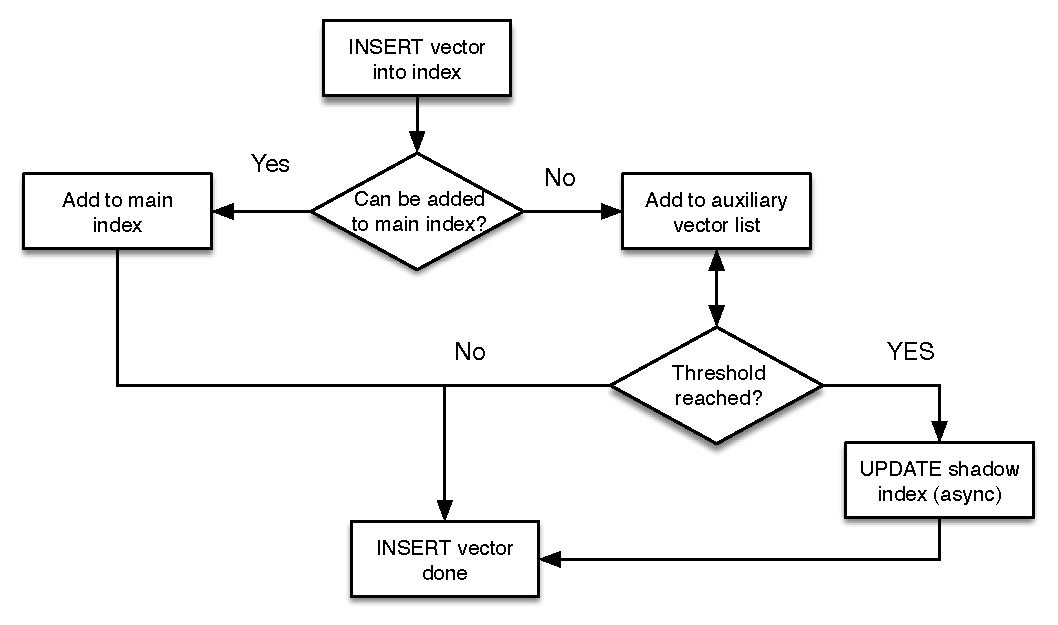
\includegraphics[width=\textwidth]{figures/adaptive_index_flow.eps}
        \label{fig:adaptive_index:flow}
    \end{subfigure}
    \caption{Adaptive index structures overview.}
    \label{fig:adaptive_index}
\end{figure}

Describe model for index management in the face of changing data (adaptive index management):

\begin{itemize}
    \item Reason about properties of secondary indexes for NNS (e.q., PQ, VA, LSH) with regards to data change
    \item Derivation of error bounds possible (e.g., usable for planning)?! Use in query planning?
    \item Systems perspective 1: How to cope with ``dirty'' indexes? Proposal: hot vs. cold index, auxilary data structure, offline optimization, see \cref{fig:adaptive_index}
    \item Systems perspective 2: On-demand index based on query workload?
\end{itemize}

\section{Generalization of Similarity Search}

Describe generalized model for similarity search:

\begin{itemize}
    \item NNS: Scan -> (Predicate) -> Distance Function -> Sort -> Limit -> (Predicate); no need for dedicated language feature aside from distance function
    \item Distance function is a binary function $D(q,v) \longrightarrow d$, $q$ and $v$ can be elements of $\mathbb{R}^d,\mathbb{C}^d$ or some other object (e.g. matrices)
    \item Different types of distance functions, depending on parameters they accept; e.g. distance between point \& point or point \& plane etc.
    \item Systems perspective 1: How enable planner to reason about distance function execution? Possible optimizations?
    \item Systems perspective 2: Concrete applications in multimedia retrieval and analytics?
\end{itemize}

\section{Cost Model for Retrieval Accuracy}
Describe cost model for execution plans with following properties:

\begin{itemize}
    \item Cost as a function of atomic costs: $f(a_{cpu}, a_{io}, a_{memory}, a_{accuracy}) \longrightarrow C$
    \item Means to estimate results accuracy and associated considerations from execution path (e.g., when using index) based on properties of the index
    \item Means to specify importance of accurate results (e.g., global, per-query, context-based i.e. when doing 1NN search) in comparison to other factors
    \item Systems perspective 1: How can such a cost model be applied during query planning and optimization?
\end{itemize}

\section{Architecture Model}

\todo[inline]{Putting everything together into a unified systems model (base on previous work + aforementioned aspects).}




